\documentclass[12pt, a4paper]{article}
\usepackage[margin=2.0cm]{geometry}
\usepackage{stmaryrd}
\usepackage{amsmath}
\usepackage{amssymb}
\usepackage{enumerate}
\usepackage{bbold}
\usepackage{dsfont}
\usepackage{wrapfig}
\usepackage{algorithm2e}
\usepackage{changepage}
\usepackage{undertilde}
\usepackage{hyperref}
\hypersetup{pdftex,colorlinks=true,allcolors=blue}
\usepackage{hypcap}
\usepackage{multicol}
\usepackage{float}
\usepackage{tikz}
\usepackage{qtree}
\usepackage[amsmath,hyperref]{ntheorem}
\usepackage{framed}
\usepackage{booktabs}
\usepackage{needspace}
\usepackage{color}
\usepackage{listings}
\usepackage{xifthen}

\setlength{\parskip}{\baselineskip}

\title{Computational Neuroscience Coursework 1}
\author{Dylan Cope (dc14470)}
\date{}

\renewcommand\vec[1]{\mathbf{#1}}
\newcommand\uvec[1]{\hat{\mathbf{#1}}}

\begin{document}

\nocite{*}
\bibliographystyle{plain}

\maketitle

\section*{Question 1}

% Simulate an integrate and fire model with the following parameters for 1 s: $\tau_m = 10 $ms, $E_L = V_r = -70$ mV, $V_t = -40$ mV, $R_m= 10$ M$\Omega$, $I_e = 3.1 $ nA. Use Euler's method with timestep $\delta t = 1$ ms. Here $E_L$ is the leak potential, $V_r$ is the reset voltage, $V_t$ is the threshold, $R_m$ is the membrane resistance, that is one over the conductance, and $\tau_m$ is the membrane time constant. Plot the voltage as a function of time. For simplicity assume that the neuron does not have a refractory period after producing a spike. [20\% of marks]. You do not need to plot spikes - once membrane potential exceeds threshold, simply set the membrane potential to $V_r$.

\begin{figure}[H]
  \centering
  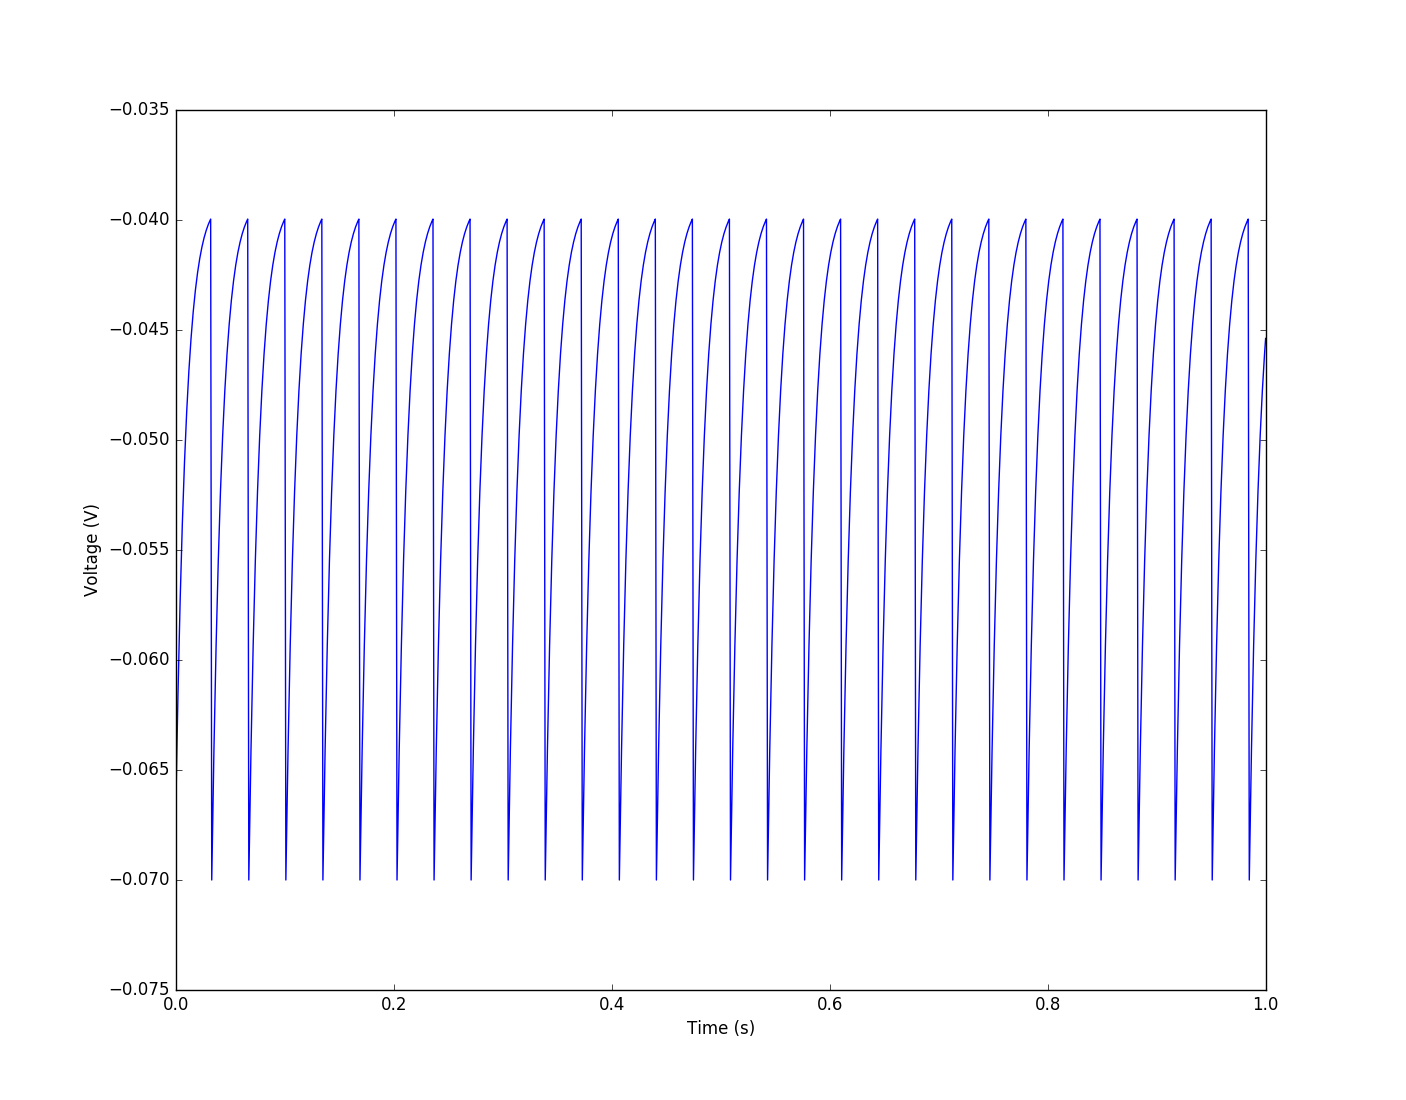
\includegraphics[width=1\linewidth]{figures/q1}
  \caption{Internal neuron voltage against time for simulating a single neuron, showing thirty spikes over the course of 1 s.}
\end{figure}

\section*{Question 2}

\section*{Question 3}

\begin{figure}[H]
  \centering
  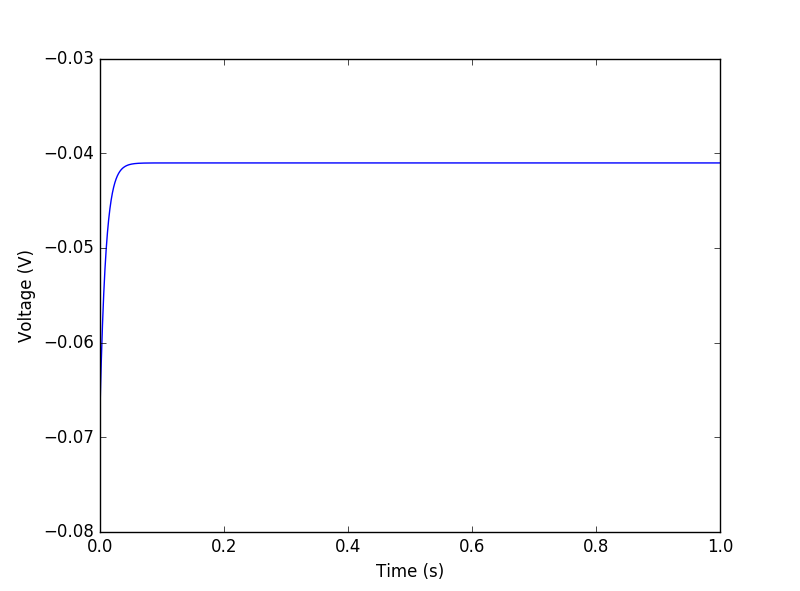
\includegraphics[width=1\linewidth]{figures/q3}
  \caption{Simulation of a neuron for 1 s with an input current of amplitude $I_e$ which is 0.1 [nA] lower than the minimum current computed in question 2.}
\end{figure}

\section*{Question 4}

\begin{figure}[H]
  \centering
  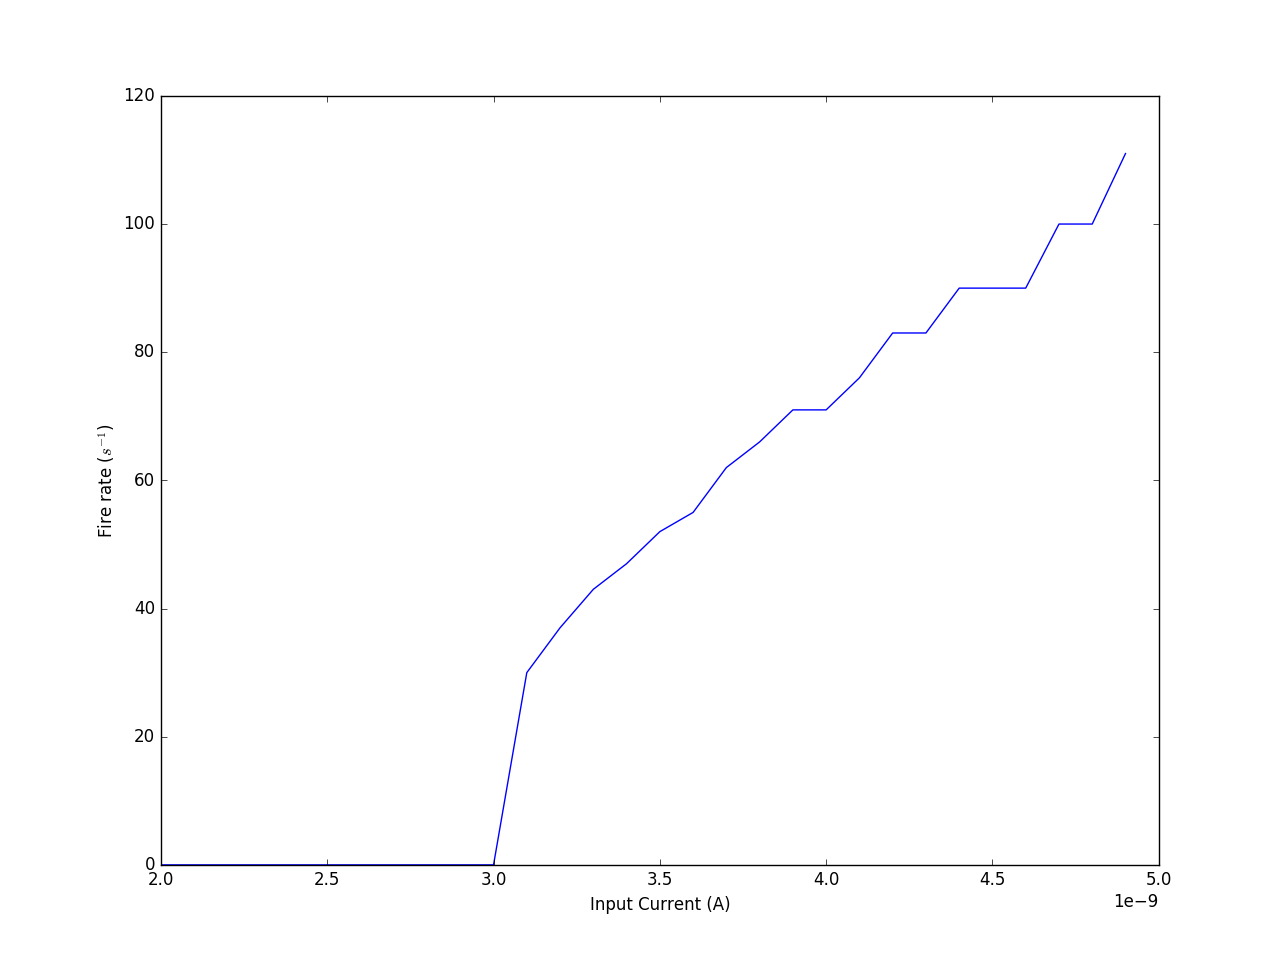
\includegraphics[width=1\linewidth]{figures/q4}
\end{figure}

\section*{Question 5}

\section*{Question 6}

\section*{Question 7}

\bibliography{dc14770}
\bibdata

\end{document}
